\documentclass[11pt,a4paper]{article}

\usepackage[english]{babel}
\usepackage[T1]{fontenc}
%\usepackage[latin1]{inputenc}

\usepackage{amsmath}
\usepackage{multirow}
%\usepackage[margin=2cm]{geometry}
\usepackage[dvipsnames]{xcolor}

\usepackage{graphicx}
\usepackage{amssymb}
\usepackage{mathrsfs}
\usepackage{subcaption}
\usepackage{setspace} 

\definecolor{AB}{rgb}{0,0.3961,0.7412}

\usepackage[bookmarksnumbered=true]{hyperref} 
\hypersetup{
     colorlinks = true,
     linkcolor = AB,
     anchorcolor = AB,
     citecolor = AB,
     filecolor = AB,
     urlcolor = AB
 }
\usepackage{enumitem}
\allowdisplaybreaks

\addtolength{\oddsidemargin}{-.8in}
\addtolength{\evensidemargin}{-.65in}
\addtolength{\textwidth}{1.68in}
\addtolength{\topmargin}{-.875in}
\addtolength{\textheight}{1.15in}

\usepackage{titlesec}
\titleformat{\section}{\fontsize{12}{14}\sc}{\thesection}{1em}{}[]
\titleformat{\subsection}{\fontsize{11}{12}\sc}{\thesubsection}{1em}{}[]
\titleformat{\subsubsection}{\fontsize{10}{11}\sc}{\thesubsection}{1em}{}[]
 
 \setlength{\parindent}{0pt}
 
\usepackage{tocloft}
\renewcommand{\cfttoctitlefont}{\sc}
\renewcommand{\cftsecfont}{\sc}
\renewcommand{\cftsubsecfont}{\sc}

\usepackage{abstract}
\renewcommand\abstractnamefont{\sc}

\usepackage[round]{natbib}

 
\begin{document}
\thispagestyle{empty}

\begin{flushleft} 
\includegraphics[width=1.0\textwidth]{headers}   \end{flushleft}

\vskip0.5cm
\begin{spacing}{2} {\Large\sc\noindent Exercise List 1}
\end{spacing}

\vfill

\begin{spacing}{1.2}
{\large\sc  Antonio Felype Ferreira Maciel - 576261}\\

{\noindent \large \sc Master's Course in Teleinformatics Engineering}\\
{\noindent \large \sc Federal University of Ceará}\\

{\noindent \large \sc TIP8300 - Nonlinear System Optimization}
\end{spacing}

\newpage 

% \tableofcontents

\newpage

%\begin{abstract}
% This report provides a concise introduction to Up-flow Anaerobic Sludge Blanket reactor, outlines its applications in Brazil, and explains the model we are using for simulations. We discuss our intentions for using this model, the challenges we are currently facing and our next steps. 
%\end{abstract}

\section*{Chapter 2 -- Convex Sets}

\begin{itemize}
    \item[\textbf{2.11}] Define the square $S = \{x \in \mathbf{R}^2 \,\vert\, 0 \leq x_i \leq 1, \, i = 1, 2\}$, and the disk $D = \{x \in \mathbf{R}^2 \, \vert \, \|x\|_2 \leq 1\}$. Are the following statements true or false?
    \item[] \begin{itemize}
        \item[(a)] $S \cap D$ is convex.
            
        A set is convex if, for every pair of point $x$ and $y \in C$ and every $\lambda \in [0, 1]$, the point $z = \lambda x + (1-\lambda)y$ also belongs to C. 

        \begin{equation*}
            S = \{(x_1, x_2) \vert 0 \leq x_1 \leq 1, 0 \leq x_2 \leq 1\}
        \end{equation*}
        
        For $x = (x_1, x_2)$ and $y = (y_1, y_2) \in S$ and $\lambda \in [0, 1]$, $z = \lambda x + (1- \lambda)y$, which means that:
        
        \begin{equation*}
            \begin{aligned}
                z_1 = & \lambda x_1 + (1- \lambda)y_1\\ 
                z_2 = & \lambda x_2 + (1- \lambda)y_2.
            \end{aligned}
        \end{equation*}

        Since $x_1$ and $x_2$ vary between 0 and 1, for every of these extremities and for the values of $\lambda$, $z_1$ and $z_2$ also belong to $S$. This way, $S$ is convex.

        \begin{equation*}
            D = \{x \in \mathbf{R}^2 \,\vert\, \Vert x \Vert_2\}
        \end{equation*}

        For $D$ to be convex, for any two points $x_1$, $x_2 \in D$ and for any $\lambda \in [0,1]$, the combination

        \begin{equation*}
            z = x_1 \lambda + (1-\lambda)x_2
        \end{equation*}

        must belong to $D$. Therefore $\Vert z \Vert_2 \leq 1$ must be true.

        Using the triangle inequality

        \begin{equation*}
            \begin{aligned}
                \Vert z \Vert_2 \leq & \, \Vert x_1 \Vert_2 \lambda + (1 - \lambda)\Vert x_2 \Vert_2\\
                \Vert x_1\lambda + (1-\lambda)\Vert_2 \leq & \, \Vert x_1 \Vert_2 \lambda + (1-\lambda) \Vert x_2\Vert_2.
            \end{aligned}
        \end{equation*}

        Since $x_1, x_2 \in D$, $\Vert x_1 \Vert_2 \leq 1$ and $\Vert x_2 \Vert_2 \leq 1$. Then, for $x_1 = x_2 = 1$

        \begin{equation*}
            \begin{aligned}
                \Vert z \Vert_2 \leq \, & \lambda(1-\lambda) = 1\\
                \Vert z \Vert_2 \leq \, & 1.
            \end{aligned}
        \end{equation*}

        This way, $D$ is also convex. Since both sets are convex and intersection preserves convexity, the sentence is \textbf{true}. $S$, in orange, and $D$ in blue are shown in Figure~\ref{fig:SD}. Their intersection is shown in Figure~\ref{fig:intersection}.
 
        \item[(b)] $S \cup D$ is convex.
        
        Union does not necessarily preserves convexity. 
        \item[(c)] $S \setminus D$ is convex.  But from Figure~\ref{fig:union}, it is possible to see that the sentence is \textbf{true}.
        
        \begin{figure}
            \centering
            \begin{subfigure}[b]{0.24\textwidth}
                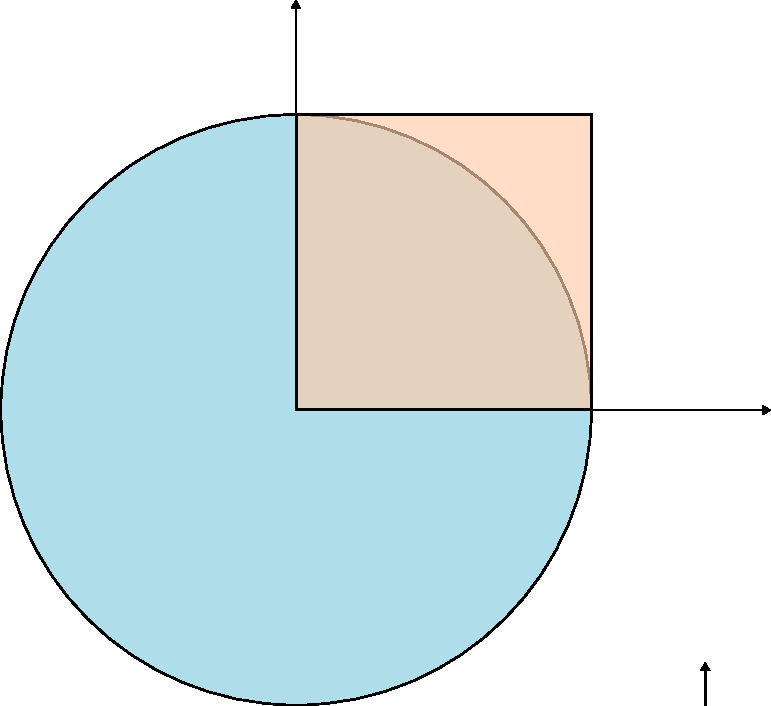
\includegraphics[width=\textwidth]{figures/SD.pdf}
                \caption{}\label{fig:SD}
            \end{subfigure}
            \begin{subfigure}[b]{0.24\textwidth}
                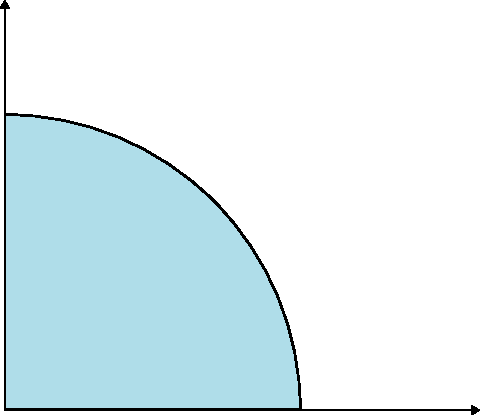
\includegraphics[width=\textwidth]{figures/intersection.pdf}
                \caption{}\label{fig:intersection}
            \end{subfigure}
            \begin{subfigure}[b]{0.24\textwidth}
                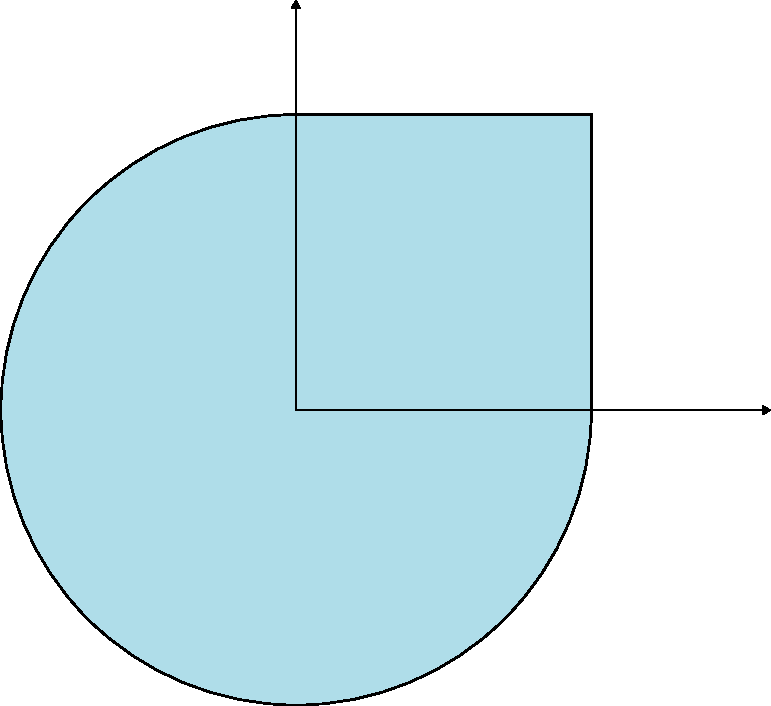
\includegraphics[width=\textwidth]{figures/SUD.pdf}
                \caption{}\label{fig:union}
            \end{subfigure}
            \begin{subfigure}[b]{0.24\textwidth}
                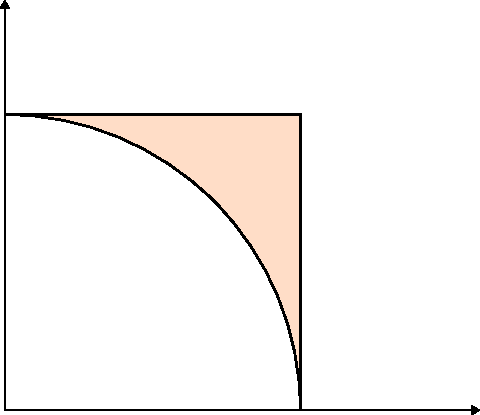
\includegraphics[width=\textwidth]{figures/difference.pdf}\label{fig:difference}
                \caption{}
            \end{subfigure}
        \end{figure}
    \end{itemize}
    \item[\textbf{2.13}] \textit{Minimal and minimum elements}. Consider the set $S = \{(0,2), (1,1), (2,3), (1,2), (4,0)\}$. Are the following statements true or false?
    \item[] \begin{itemize}
        \item[(a)] (0,2) is the minimum element of $S$.
        \item[(b)] (0,2) is a minimal element of $S$.
        \item[(c)] (2,3) is a minimal element of $S$.
        \item[(d)] (1,1) is a minimal element of $S$.
    \end{itemize}
        Here, minimum and minimal are with respect to the nonnegative orthant $K = \mathbf{R}_+^2$.
    \item[\textbf{2.16}] \textit{Generalized inequality}. Let $K = \{(x_1,x_2) \, \vert \, 0 \leq x_1 \leq x_2\}$. Are the following statements true or false?
    \item[] \begin{itemize}
        \item[(a)] $(1,3) \preceq_K (3,4)$.
        \item[(b)] $(-1,2) \in K^*$.
        \item[(c)] The unit circle (\textit{i.e.}, $\{x \, \vert \, \|x\|_2 = 1\}$) does not contain a minimum element with respect to $K$.
        \item[(d)] The unit circle does not contain a minimal element with respect to $K$.
    \end{itemize}
\end{itemize}

\section*{Chapter 3 -- Convex Functions}

\begin{itemize}
    \item[\textbf{3.33}] \textit{DCP rules}. The function $f(x,y) = \sqrt{1 + x^4/y}$, with $\textbf{dom} f = \mathbf{R}\times\mathbf{R}_{++}$, is convex. Use disciplined convex programming (DCP) to express $f$ so that it is DCP convex. You can use any of the following atoms
    \item[]\begin{itemize}
        \item[] \texttt{inv\_pos(u)}, which is $1/u$, with domain $\mathbf{R}_{++}$
        \item[] \texttt{square(u)}
        \item[] \texttt{sqrt(u)}
        \item[] \texttt{geo\_mean(u,v)}
        \item[] \texttt{quad\_over\_lin(u,v)}
        \item[] \texttt{norm2(u,v)}
    \end{itemize}

    You may also use addition, subtraction, scalar multiplication, and any constant functions. Assume that DCP is sign-sensitive, \textit{e.g.}, \texttt{square(u)} is known to be increasing in $u$ for $u \geq 0$.

    \item[\textbf{3.38}] \textit{Curvature of some functions}. Determine the curvature of the functions below. Your responses can be: affine, convex, concave, and none (meaning, neither convex nor concave).
    \item[] \begin{itemize}
        \item[(a)] $f(x) = \min\{2,x,\sqrt{x}\}$, with $\textbf{dom}\, f = \mathbf{R}_+$
        \item[(b)] $f(x) = x^3$, with $\textbf{dom} \, f = \mathbf{R}$
        \item[(c)] $f(x) = x^3$, with $\textbf{dom} \, f = \mathbf{R}_{++}$
        \item[(d)] $f(x,y) = \sqrt{x \min\{y,2\}}$, with $\mathbf{dom} \, f = \mathbf{R}_+^2$
        \item[(e)] $f(x,y) = (\sqrt{x} + \sqrt{y})^2$, with $\textbf{dom} \, f = \mathbf{R}_+^2$
        \item[(f)] $f(\theta) = \log \det \theta - \textbf{tr}(S\theta)$, with $\textbf{dom} \, f = \mathbf{S}_{++}^n$, and where $S \succ 0$
    \end{itemize}

    \item[\textbf{3.55}] State wether each of the following statement is true or false.
    \item[] \begin{itemize}
        \item[(a)] $f(x) = (x^2 + 2)/(x + 2)$, with $\textbf{dom}\, f = (-\infty, -2)$ is convex.
        \item[(b)] $f(x) = 1/(1-x^2)$, with $\textbf{dom} \, f = (-1,1)$ is convex.
        \item[(c)] $f(x) = 1/(1-x^2)$, with $\textbf{dom} \, f = (-1,1)$ is log-convex.
        \item[(d)] $f(x) = \cosh x = (e^x + e^{-x})/2$ is convex.
        \item[(e)] $f(x) = \cosh x$ is log-concave.
        \item[(f)] $f(x) = \cosh x$ is log-convex.
    \end{itemize}
\end{itemize}

\section*{Chapter 4 -- Convex optimization functions}

\begin{itemize}
    \item[\textbf{4.3}] \textit{Formulating constraints in CVX*.} Below we give several convex constraints on scalar variables $x$, $y$, and $z$. Express each one as a set of valid constraints in CVX*. (Directly expressing them in CVX* will lead to invalid constraints.) You can also introduce additional variables, if needed.
    
    Check your reformulations by creating a small problem that includes these constraints, and solving it using CVX*. Your test problem doesn't have to be feasible; it's enough to verify that CVX* processes your constraints without error.

    \begin{itemize}
        \item[(a)] $1/x + 1/y \leq 1, \, x \geq 0, \, y \geq 0$.
        \item[(b)] $xy \geq 1, \, x \geq 0, \, y \geq 0$.
        \item[(c)] $(x+y)^2 / \sqrt{y} \leq x - y + 5$ (with implicit constraint $y \geq 0$).
        \item[(d)] $x + z \leq 1 + \sqrt{xy - z^2}, \, x \geq 0, \, y \geq 0$ (with implicit constraint $y > 0$).
    \end{itemize}

    \item[\textbf{4.4}] \textit{Optimal activity levels}. Solve the optimal activity level problem described in exercise 4.17 in \textit{Convex Optimization}, for the instance with problem data
    
    \begin{equation*}
        A = \begin{bmatrix}
            1 & 2 & 0 & 1\\
            0 & 0 & 3 & 1\\
            0 & 3 & 1 & 1\\
            2 & 1 & 2 & 5\\
            1 & 0 & 3 & 2
        \end{bmatrix},
        \qquad
        e^{max} = \begin{bmatrix}
            100\\
            100\\
            100\\
            100\\
            100
        \end{bmatrix},
        \qquad
        p = \begin{bmatrix}
            3\\
            2\\
            7\\
            6
        \end{bmatrix},
        \qquad
        p^{disc} = \begin{bmatrix}
            2\\
            1\\
            4\\
            2
        \end{bmatrix},
        \qquad
        q = \begin{bmatrix}
            4\\
            10\\
            5\\
            10
        \end{bmatrix}
    \end{equation*}

    You can do this by forming the LP you found in your solution of exercise 4.17, or more directly, using CVX*. Give the optimal activity levels, the revenue generated by each one, and the total revenue generated by the optimal solution. Also, give the average price per unit for each activity level, \textit{i.e.}, the ratio of the revenue associated with an activity, to the activity level. (These numbers should be between the basic and discounted prices for each activity). Give a \textit{very brief} story explaining, or at least commenting on, the solution you find.

    \item[\textbf{4.24}] \textit{CVX implementation of a concave function}. Consider the concave function $f: \mathbf{R} \to \mathbf{R}$ defined by
    
    \begin{equation*}
        f(x) = \begin{cases}
            (x+1)/2 & x>1\\
            \sqrt{x} & 0 \leq x \leq 1,
        \end{cases}
    \end{equation*}

    with $\textbf{dom} \, f = \mathbf{R}_{++}$. Give a CVX implementation of $f$, via a partially specified optimization problem. Check your implementation by maximizing $f(x) + f(a - x)$ for several interesting values of $a$ (say, $a = -1$, $a = 1$, and $a = 3$).
\end{itemize}

\end{document}
